% Two-page revision: fixed-rank motivation, scale matching, and empirical ERG gaps.
% One compact SETOL citation; no separate bibliography in the standalone insert.
\subsection{Reconciling the SETOL and MLE normalizations}
\label{sxn:meanlog_gauge}

SETOL and the power-law fit choose different spectral reference scales,
so explaining their agreement near marginality requires both a reason
for scaling eigenvalues by $M$ and a test of whether the two rules select
the same ECS.
SETOL uses $\lambda/M$; the fit uses
$\lambda/\PLstart$.

\begin{tcolorbox}[marginalbox,title=\textbf{Matching the normalizations}]
  We have two different normalizations
\eqtight{
\text{SETOL: }\tilde{\lambda}_{\mathrm ECS}:=\frac{\lambda}{M},
\qquad
\text{MLE: }\tilde{\lambda}_{\mathrm PL}:=\frac{\lambda}{\PLstart}.
}
At $\alpha=2$, matching requires $M\simeq e\PLstart$.
\takeaway{RG scale invariance motivates $1/M$.
Why these normalizations align remains an open question.}
\end{tcolorbox}

\paragraph{Why marginality motivates $1/M$.}
A stable marginal tail motivates division by matrix size because a fixed
upper rank moves to proportionally larger eigenvalues as the spectrum grows.
Let the probability-normalized spectrum have survival tail
$\overline F(\lambda)\simeq C\lambda^{1-\alpha}$, with unchanged amplitude
$C$ and common units across sizes.
The characteristic location of the $r$th largest eigenvalue obeys
\begin{equation}
\begin{aligned}
r&\simeq M\overline F(\lambda_{(r)}),
&\lambda_{(r)}&\simeq(CM/r)^{1/(\alpha-1)},\\
\alpha&=2:
&\frac{\lambda_{(r)}}{M}&\simeq\frac Cr.
\end{aligned}
\label{eq:fixed_rank_marginal_scaling}
\end{equation}
Doubling $M$ therefore doubles this fixed-rank scale while leaving
its normalized position unchanged (Figure~\ref{fig:fixed_rank_scaling}).

\begin{center}
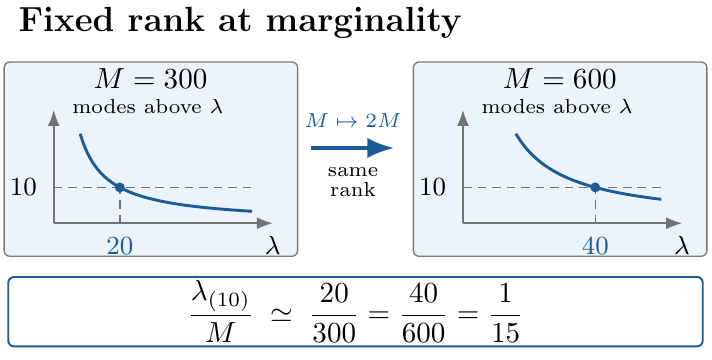
\includegraphics[width=\columnwidth]{figures/fixed_rank_scaling.png}
\vspace{-0.65em}
\captionof{figure}{\textbf{Division by $M$ preserves a fixed upper-rank scale.}
For the illustrative tail $\overline F(\lambda)=2/(3\lambda)$,
doubling $M$ moves the threshold with ten expected exceedances
from $20$ to $40$.  The normalized scale is unchanged.
This is an analytic illustration, not a measured width sweep.}
\label{fig:fixed_rank_scaling}
\end{center}

This scaling applies to fixed upper ranks away from an endpoint;
a fixed fraction $r/M$ instead gives a size-independent threshold.
The retained count $M_{\mathcal R}$ normalizes ECS averages.
Using it as an eigenvalue denominator requires a separate RG argument,
because truncation changes the cutoff and retained fraction.

% Standalone layout only; these hooks are inert in the full draft.
\ifdefined\RGTheoryColumnBreak\RGTheoryColumnBreak\fi
\paragraph{How the MLE estimator sets the scale.}
The ~\WW tool fits the power law tail using a Maximum Likelihood Estimator (MLE),
which itself is defined by estimating the mean log-eigenvalue of the tail
\begin{equation}
\left\langle\log\tilde{\lambda}_{\mathrm{PL}}\right\rangle_{\rm MLE}=\frac{1}{\hat\alpha-1},
\qquad
G_{\rm PL}=\PLstart e^{1/(\hat\alpha-1)}.
\label{eq:mle_logmean_bridge}
\end{equation}
where $G_{\rm PL}$ is the \emph{retained geometric mean}.
At $\hat\alpha=2$, the expected or mean log-eigenvalue is
$\langle \ln \tilde{\lambda}_{\mathrm{PL}}\rangle_{\rm MLE}=1.0$ when
the tail eigenvalues $\tilde{\lambda}_{\mathrm{PL}}$ are normalized by $\PLstart$.
In $G_{\rm PL}$, the factor $e$ moves the mean log-ratio from $1\rightarrow 0$.
The SETOL condition places $G_{\mathcal R}$ near $M$.
Agreement therefore requires $G_{\rm PL}\simeq G_{\mathcal R}\simeq M$;
the scale-invariance argument here alone does not impose this equality,
but it is a start.

The physical matching hypothesis identifies the marginal PL tail with
the persistent correlations that survive the RG construction.
If the two selection rules approach the same effective modes and mean
log in common units, their geometric means approach one another.
This provides a physical reason to expect a small gap near marginality.
We have no mathematical proof that the two selections converge,
and the fixed-rank argument does not fix their relative amplitude.
Instead, we rely on empirical evidence.

\paragraph{What marginality balances.}
The same marginal law gives equal logarithmic bands equal expected
energy because declining mode counts compensate for increasing
individual energies.
For probability density $\rho(\lambda)=C\lambda^{-2}$, the mean
energy $\lambda/M$ per log interval is
\begin{equation}
\frac{dE_M}{d\log(\lambda/M)}
=\frac{\lambda^2\rho(\lambda)}{M}=\frac CM.
\label{eq:energy_per_log_band}
\end{equation}
Figure~\ref{fig:normalization_band_theory} depicts this balance,
while Figure~\ref{fig:normalization_checkpoint_audit}(a) shows
this for a typical well trained layer (describe below).

\begin{center}
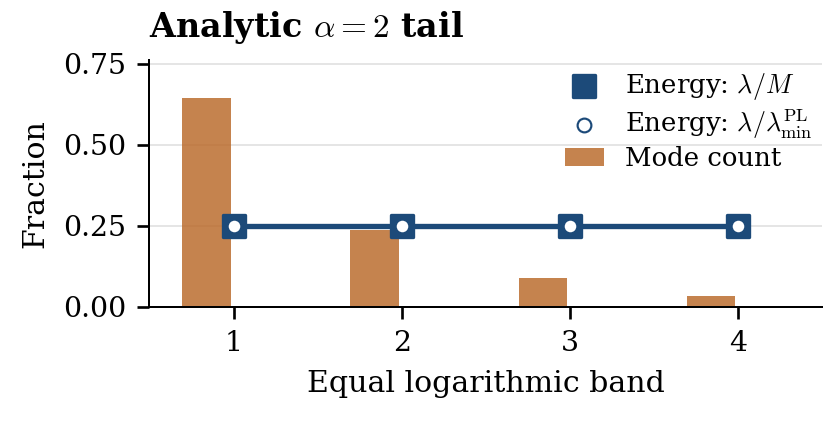
\includegraphics[width=\columnwidth]{figures/log_band_theory.png}
\vspace{-0.65em}
\captionof{figure}{\textbf{Marginality balances energy under either reference.}
An analytic $\alpha=2$ density on four equal logarithmic bands
has decreasing count fractions and equal energy fractions.
Both energy curves use the same modes and divide by the energy in
the plotted window; their reference scales cancel.}
\label{fig:normalization_band_theory}
\end{center}

\begin{figure*}[!t]
\centering
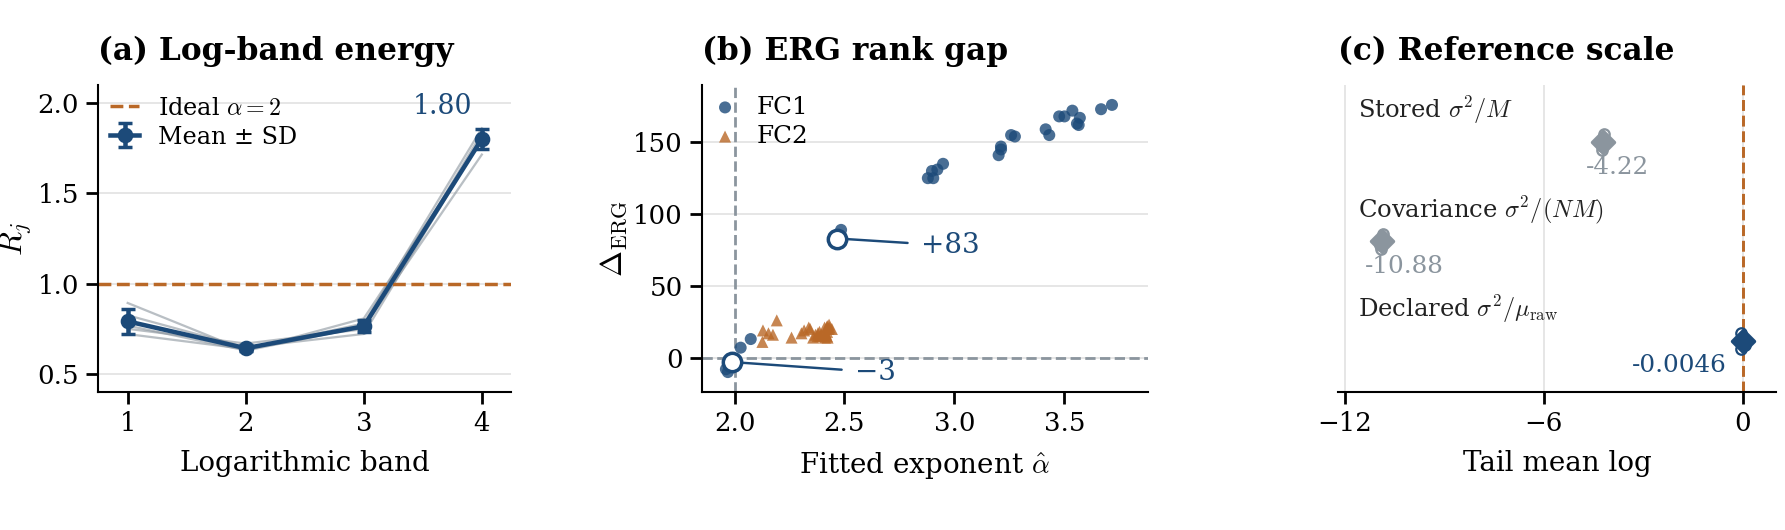
\includegraphics[width=\textwidth]{figures/checkpoint_bands_gaps_scales.png}
\vspace{-0.8em}
\caption{\textbf{Trained checkpoints show approximate matching and substantial exceptions.}
(a) Five FC1 tails at learning rate $0.32$ have
$\overline{\hat\alpha}=2.0036$ but unequal log-band energies.
$R_j$ divides each band's energy by that checkpoint's mean band energy;
error bars are between-seed standard deviations.
(b) ERG rank gaps for both hidden layers of all 30 checkpoints; labels
mark the paired seed-4 FC1 examples.
(c) The same five FC1 tails have different mean-log offsets under the
stored, covariance, and declared full-spectrum conventions.
The archive is an independent MNIST protocol replication.}
\label{fig:normalization_checkpoint_audit}
\end{figure*}

\ifdefined\RGDataPageBreak\RGDataPageBreak\fi
\paragraph{Which normalization the checkpoints test.}
Checkpoint comparisons require a fixed spectral convention because the
saved weight scale determines the trace-log reference.
Similar to the experiments in~\cite{MartinHinrichsSETOL2025}.
we examine $30$ checkpoints of a
$784\to300\to100\to10$ MNIST MLP: plain SGD, batch size $32$,
six learning rates $0.01$--$0.32$, and five seeds.
The archived Frobenius convention divides
$\lambda_i^{\rm raw}=\sigma_i(\W)^2$ by its full-spectrum mean
$\mu_{\rm raw}=M^{-1}\sum_i\lambda_i^{\rm raw}$.
In SETOL coordinates this becomes
\begin{equation}
\lambda_i:=\frac{M}{\mu_{\rm raw}}\lambda_i^{\rm raw},
\qquad
\tilde{\lambda}_{\mathrm{ECS},i}:=\frac{\lambda_i}{M}.
\label{eq:declared_checkpoint_conversion}
\end{equation}
The cutoff undergoes the same conversion.

The fitted tail's mean-log offset tests whether its center agrees
with the declared reference:
\begin{equation}
\Delta_{\rm mean-log}:=\left\langle\log\tilde{\lambda}_{\mathrm{ECS}}\right\rangle_{\rm MLE}
=\frac{1}{\hat\alpha-1}
-\log\frac{M}{\PLstart}.
\label{eq:reconcile_normalization_mismatch}
\end{equation}
In Figure~\ref{fig:normalization_checkpoint_audit}(a), the first $3$ bands
are fairly flat, where as the last band diverges up (presumably
due to the finite cut-off at $\lambda_{max}$).

More directly, Figure~\ref{fig:normalization_checkpoint_audit}(b) shows that
the ERG rank gap shrinks to $\Delta_{ERG}\rightarrow 0$ as $\alpha \rightarrow 2$.
Additional, similar results are reported in~\cite{MartinHinrichsSETOL2025}.

Finally, Figure~\ref{fig:normalization_checkpoint_audit}c) shows that trace-log agreement depends on the spectral normalization.
Dividing $\lambda_{i}^{\rm raw}$ by the full-ESD mean $\mu_{\rm raw}$
gives mean $\Delta_{\rm mean-log}=-0.0046$ and
mean $|\Delta_{\rm mean-log}|=0.051$ for the five FC1 fits at learning rate $0.32$.
These small offsets place the tail geometric means near the full-ESD arithmetic means.
Dividing instead by $M=300$ gives a mean offset of $-4.219$; the covariance convention $\sigma_i^2/(NM)$, with $N=784$, gives $-10.883$.

\paragraph{Why the ERG rank gap can remain nonzero.}
We define the \emph{ERG rank gap} as
\begin{equation}
\Delta_{\rm ERG}:=M_{\mathcal R}-M_{\rm PL}.
\label{eq:erg_rank_gap}
\end{equation}
In other models, the ERG rank gap persists and can be as large as $50$.
For nested upper tails, its sign agrees with the normalized cutoff difference 
$\Delta\tilde{\lambda}_{\min}:=\PLstart/M-\ECSstart$ used in SETOL,
although the units differ.
When a zero crossing exists, a positive fitted-tail log sum calls for
adding lower modes below the reference; a negative sum calls for
removing low modes.  The normalization and cutoff region therefore
help determine the gap, alongside the exponent.

\ifdefined\RGDataColumnBreak\RGDataColumnBreak\fi
\paragraph{Small and large gaps in the same training setup.}
The recovered checkpoints show a useful near-marginal correspondence
without exact agreement of the two retained spaces.
For FC1 with seed $4$, the original selections give
\begin{center}
\small
\begin{tabular}{c@{\quad}c@{\quad}r@{\quad}r@{\quad}r}
Learning rate & $\hat\alpha$ & $M_{\rm PL}$ & $M_{\mathcal R}$ & $\Delta_{\rm ERG}$\\
\hline
$0.16$ & $2.468$ & $119$ & $202$ & $+83$\\
$0.32$ & $1.987$ & $162$ & $159$ & $-3$
\end{tabular}
\end{center}
A three-mode difference between roughly $160$-mode tails is close
physical agreement; an $83$-mode difference is substantial.
Across the five near-marginal FC1 fits, gaps span $[-10,+13]$
despite their signed mean of $-0.2$.

The observed ERG rank gap usually approaches zero from above as $\alpha \rightarrow 2$.
All $57$ hidden-layer fits with $\hat\alpha\ge2$ have positive rank gaps;
the three with $\alpha < 2$ have negative gaps (Figure~\ref{fig:normalization_checkpoint_audit}b).
SETOL reports a similar approach toward zero from above, crossings below
$\alpha=2$, with a few exceptions: some layers with $\alpha\approx 2$ have large cutoff gaps,
and some DenseNet layers with $\alpha < 2$ retain positive gaps.

The same near-marginal checkpoints retain uneven band energies, so
center matching does not establish exact spectral scale invariance.
Their four mean relative energies,
$(0.792,0.643,0.764,1.801)$, survive scalar rescaling
(Figure~\ref{fig:normalization_checkpoint_audit}a).
Why do these differ ? Possible causes include sampling effects,
conditioning on $\lambda_{max}$, and departures an ideal power law.

More broadly, we still need to idenify how and why the scale convention and RG
transformation that align the independently selected  ECS and power law tail.
This is left to future work.

